\documentclass[10pt,a4paper]{article}
\usepackage[utf8]{inputenc}
\usepackage[T1]{fontenc}
\usepackage{geometry}
\usepackage[italian]{babel}
\usepackage{graphicx}
\usepackage{caption}
\usepackage{xcolor}
\usepackage{enumitem}
\usepackage{newtxtext,newtxmath}

\geometry{a4paper, margin=2.5cm, top=2.5cm, bottom=2.5cm} 
\usepackage{fancyhdr}
\pagestyle{fancy}
\fancyhf{} 
\renewcommand{\headrulewidth}{0pt}
\renewcommand{\footrulewidth}{0.5pt}
\fancyfoot[L]{\small Relazione Progetto Sistemi Intelligenti}
\fancyfoot[R]{\small Pagina \thepage}

\begin{document}

    \begin{center}
        {\huge \textbf{Relazione Progetto Sistemi Intelligenti per Internet}} \\ 
        \vspace{4mm}
        \rule{\textwidth}{1.5pt} 
        \vspace{6mm}
    \end{center}

    \noindent Questo progetto tratta un sistema software con interfaccia Web, in particolare un Decision Support System, che
    permette ad un oncologo di caricare delle analisi cliniche di un paziente in cura, e lo aiuta a capire se il
    paziente è oncologico oppure no, e con che probababilità. Tale progetto, si basa sul linguaggio di programmazione
    Python, poiché è il linguaggio più utilizzato nell'ambito del Machine Learning, che è ciò che si basa la maggior
    parte progetto. Inoltre, implementa anche la XIA, che spiega il motivo della decisione presa dal sistema.

    \section*{Architettura software utilizzata}
        Tale applicazione è strutturata secondo il paradigma Object-Oriented e l'architettura Client-Server, garantendo 
        una rigorosa Separation of Concerns (SoC) attraverso il pattern Model-View-Controller (MVC). \\
        Il Model si occupa della persistenza dei dati e della logica di dominio: è implementato tramite il DBMS 
        open-source PostgreSQL (molto usato in ambito medico) e usa il modello di Machine/Deep Learning per l'inferenza 
        dei dati. \\
        La View è responsabile della presentazione e dell'interazione con l'utente: in particolare è sviluppata tramite il 
        framework Streamlit, che rende del tutto invisibile agli sviluppatori la complessità di HTML, CSS e JavaScript,
        fornendo un'interfaccia reattiva ed soprattutto intuitiva. Ciò viene arricchito dalla visualizzazione di grafici 
        per la eXplainable AI (XAI) e referti in PDF: in questo modo l'utente può capire i motivi che hanno portato alla
        decisione del modello: infatti, questo passa da essere un sistema di Intelligenza Artificiale puro ad un vero e
        proprio Sistema di Supporto alle Decisioni. \\
        Il Controller, che è stato sviluppato in Python 3.12, è il direttore di orchestra del sistema vero e proprio: 
        difatti gestisce le richieste da parte del frontend, interroga il database, elabora i dati tramite l'IA e invoca
        anche dei processi esterni per generare il referto in PDF, sfruttando un compilatore LaTeX, ottimo per la
        generazione di documenti PDF.\\
        L'intera architettura è containerizzata tramite Docker,pratica molto comune in ambiente di sviluppo, poiché 
        assicura la massima portabilità, isolamento e scalabilità dell'ambiente di esecuzione.
    
    \subsection*{Entità e relazioni}
        \begin{center}
            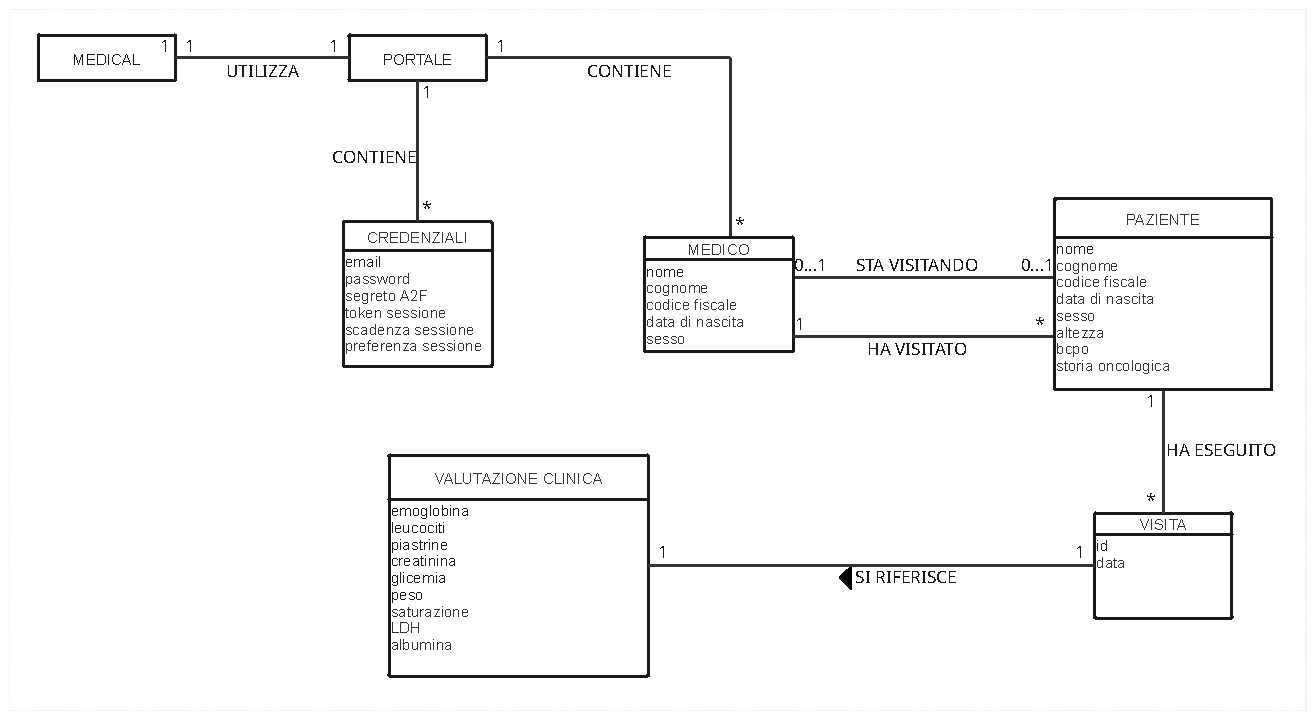
\includegraphics[width=0.8\textwidth]{immagini/dominio.pdf}
            \vspace{2mm} % Un piccolo spazio extra tra immagine e didascalia
            \captionof{figure}{Modello di dominio}
            \label{fig:dominio} % Label per citare la figura nel testo con \ref{fig:dominio}
        \end{center}
        Il sistema deve poter memorizzare ogni medico, con delle credenziali, a cui viene associata una email. Ogni
        medico contiene un nome, un cognome, una data di nascita, un codice fiscale ed il sesso. Le credenziali invece
        contengo, l'email, la password criptata, dei token per l'autentificazione a due fattori e per la sessione, per
        evitare logout al reload della pagina e gestire la sessione per il sito. \\
        Il medico può selezionare ogni paziente che ha in cura, che inserisce il suo nome, cognome, codice fiscale, data
        di nascita, sesso, altezza, se è un soggetto BCPO (BroncoPneumopatia Cronica Ostruttiva) e se in passato ha avuto
        dei precedenti oncologici. Il paziente è in cura presso un solo medico. \\
        Il medico esegue delle visite al paziente, in cui viene memorizzata la data ed un identificativo per essere memorizzata.
        A questo punto, ad ogni visita gli viene associata, una propria valutazione clinica, in cui vengono memorizzati questi
        valori non obbligatori eccetto per il primo: peso, emoglobina, leucociti, piastrine, creatinina, glicemia, saturazione,
        LDH ed albumina.\\
    \subsection*{Caso d'uso "processa analisi"}
        Il sistema possiede diversi casi d'uso, come l'inserimento del nuovo paziente, di una nuova visita, la registrazione di un nuovo medico. Tuttavia,
        quello soggetto di studio è quello della predizione.\\
        \textit{Caso d'uso: Processa Analisi}
        \begin{enumerate}
            \item Un medico vuole eseguire la predizione delle analisi effettuate ad un paziente.
            \item Il medico esegue il login, con l'A2F ed il Sistema mostra i suoi dati e i pazienti in cura.
            \item Il medico seleziona il paziente a cui vuole effettuare la predizione: il Sistema mostra la cartella clinica e l'elenco delle visite effettuate.
            \item Il medico seleziona la predizione delle analisi, il Sistema carica le analisi e avvia il modello di Machine Learning, che invia al Sistema il risultato della predizione.
            \item Il medico può scaricare il referto in formato PDF.
        \end{enumerate}
        Di seguito, viene mostrato il seguente diagramma delle classi, dove GestoreDB permette la connessione con il DBMS.
        \begin{center}
            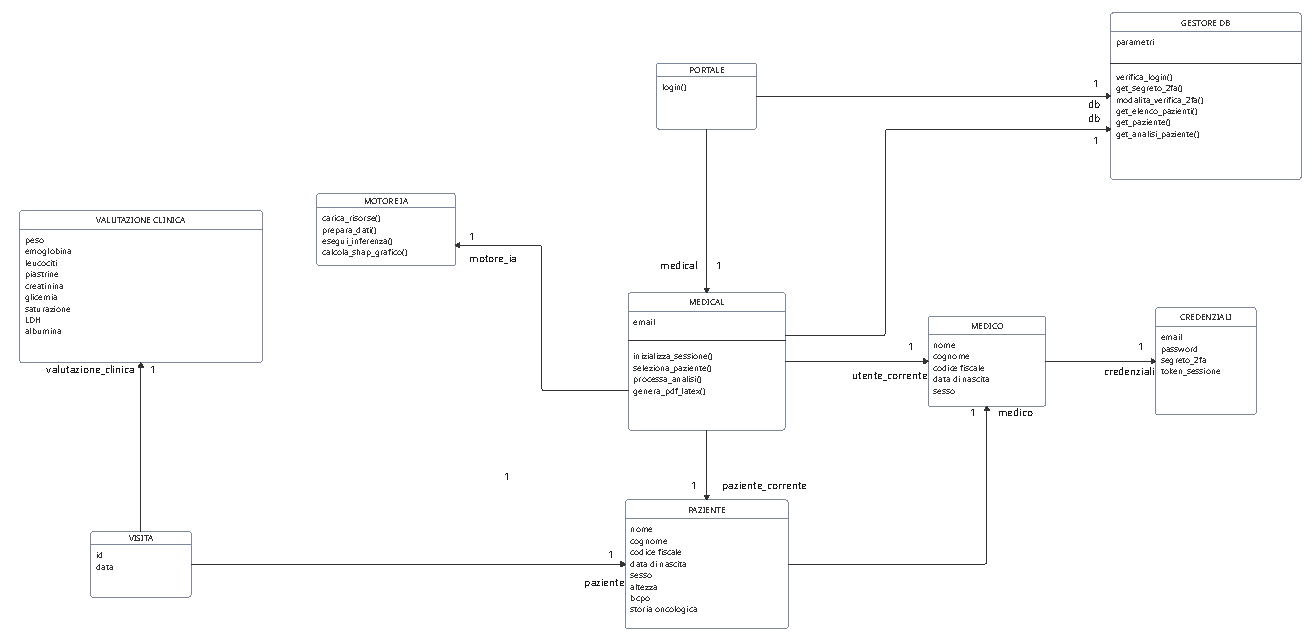
\includegraphics[width=\textwidth, height=20\textheight, keepaspectratio]{immagini/classi.pdf}
            \vspace{2mm} 
            \captionof{figure}{Diagramma delle classi}
            \label{fig:classi}
        \end{center}
        Adesso verrano raffigurati i diagrammi di sequenza di sistema, per ogni scenario di successo.
        

\end{document}